%----------------------------------------------------------------------------
\section{Irodalomkutatás}
%----------------------------------------------------------------------------

% \subsection{Generatív modellek csoportosítása}

% \subsubsection{Supervised learning}

A gépi tanulási modellek csoportosíthatók a feladat típusa alapján: megkülönböztetünk felügyelt és felügyelet nélküli, illetve megerősítéses tanulást.

\begin{figure}[h]
	\centering
	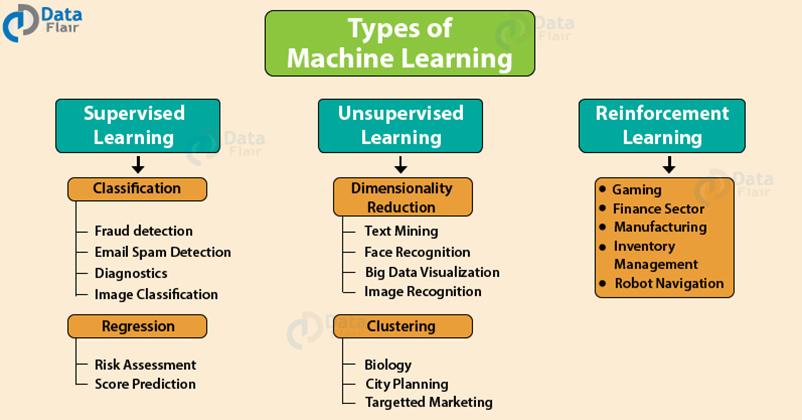
\includegraphics[width=1\columnwidth]{figures/machine_learning_types.png}
	\caption{abra alatti szoveg}
\end{figure}

A felügyelt tanulásnál ismerjük a tanító mintakészlethez tartozó célértékeket, elvárt kimeneteket. Az ilyen adatot címkézett adatot címkézettnek nevezzük. A felügyelt tanulás célja egy olyan funkció elsajátítása, amely az adatok mintája és a kívánt kimenetek alapján a legjobban közelíti az adatokban megfigyelhető bemenet és kimenet közötti kapcsolatot. A felügyelet nélküli tanulásnak viszont nincsenek címkézett kimenetei, ezért célja az adathalmazon belső szerkezetének megtanulása. Az ilyen modelleket címkézett adatokon tanítanak be, majd a modell által korábban nem látott új mintákra képest helyes becslést adni. A felügyelt tanulásnak két alkategóriája van, a regresszió és az osztályozás vagy más nével klasszifikáció. Osztályozás esetén a kimenetet két vagy több osztályba kell csoportosítani. Ha az algoritmus a bemenetet két különböző osztályba sorolja, akkor ezt bináris osztályozásnak nevezzük, míg a több mint két osztály közötti választást többosztályos osztályozásnak nevezzük. Ezzel szemben a regressziós algoritmusokat folytonos értékek előrejelzésére használják, mint például az ár, a fizetés és az életkor.
 
A felügyelet nélküli tanulás esetén a megfigyelésekhez nem áll rendelkezésre elvárt célérték (azaz felügyelet). Célunk, hogy az adatok közt mintázatokat, összefüggéseket azonosítsunk. A tanítás itt a kérdéses mintázat/összefüggés definícióját jelenti, ami általában számos mérnöki iteráció után alakul ki. felügyelet nélküli tanulás alkalmazható többek között klaszterezési feladatok megoldására, dimenziócsökkentésre, asszociációs feladatokra, anomália detektálásra, illetve generatív modelleknél is.

% In Supervised Learning, we train the machine using data that is well “labeled”. It means the data is already tagged with the correct answer. A supervised learning algorithm learns from labeled training data and predicts outcomes for unforeseen data. There are two subcategories of supervised learning, Regression and Classification. Classification means to group the output into a class. If the algorithm tries to label input into two distinct classes, it is called binary classification. Selecting between more than two classes is referred to as multiclass classification. On the other hand, Regression Algorithms are used to predict continuous values such as price, salary, and age.

%--------------
% Felügyelt tanulás (supervised learning): a tapasztalatok itt egy megfigyelés/adat és a hozzá tartozó elvárt célérték. A tapasztalatok halmaza egyben adott, ezt hívjuk tanító adatbázisnak (training dataset). A cél, hogy ez alapján olyan modellt tanuljunk ami korábban nem látott példákon is helyesen működik. Példa alkalmazás: ügyfélszolgálatra érkező e-mail panaszleveleket akarunk automatikusan továbbítani a megfelelő munkatárshoz, aki meg tudja válaszolni azt. Ehhez rendelkezésre áll több ezer e-mail a múltból (adat) és, hogy melyik munkatárshoz kellett irányítani a levelet (elvárt célérték). Ebből a tanító adatbázisból kell megtanulnunk egy modellt, ami a holnap érkező e-maileket a lehető legnagyobb pontossággal automatikusan a megfelelő munkatárshoz irányítja.  
% Felügyelet nélküli tanulás (unsupervised learning): A megfigyelésekhez nem áll rendelkezésre elvárt célérték (azaz felügyelet). Célunk, hogy az adatok közt mintázatokat/összefüggéseket azonosítsunk. A tanítás itt a kérdéses mintázat/összefüggés definícióját jelenti, ami általában számos mérnöki iteráció után alakul ki.  Példa alkalmazás: a vállalat ügyfeleiről rendelkezésre állnak azok múltbeli tranzakcióinak adatai. Találjunk olyan ügyfél csoportokat, akik hasonlóan viselkednek anélkül, hogy a viselkedési csoportokat előre megadnánk! Figyelem, mérnöki feladat, hogy két tranzakciósorozat hasonlóságt leírjuk!  
% Megerősítéses tanulás (reinforcement learning): a rendszer folyamatosan akciókat hajt végre, néha kap megerősítést, hogy mennyire jól csinálja a feladatát, és ezekből a megerősítésekbő folyamatosan tanul.  Példa alkalmazás: Robotot tanítunk büntetőt rúgni fociban. A robot csak a büntetőrúgás végén kap visszajelzést, hogy sikeres volt-e. Ebből kell saját magának kialakítani a mozgássorozatot, amire majd megint kap megerősítést (aktív tanulás).
%-------------- (https://www.inf.u-szeged.hu/~rfarkas/ML20/alapfogalmak.html)

% Unsupervised Learning is a machine learning technique, where the model does not need any supervision. Instead, we need to allow the model to work on its own to discover information. It mainly deals with the unlabelled data. Density estimation, dimensionality reduction, and clustering and some of the main applications of unsupervised learning.

% In Machine learning, supervised learning methods are used when the objective is to learn mapping between the attributes and the target in the data. When the objective is to identify the underlying structure or the pattern in the data, unsupervised learning methods are useful. Some of the popular unsupervised learning methods are Clustering, Dimensionality reduction, Association mining, Anomaly detection and Generative models. Each of these techniques have a different pattern recognition objective such as identifying latent grouping, identifying latent space, finding irregularities in the data, density estimation or generating new samples from the data. 

%----------------------------------------------------------------------------
% \subsubsection{Generative vs discriminative modeling}

A gépi tanulási modelleket feladatuk szerint két további alkategóriába sorolhatjuk: generatív és diszkriminatív modellek. 

\begin{figure}[h]
	\centering
	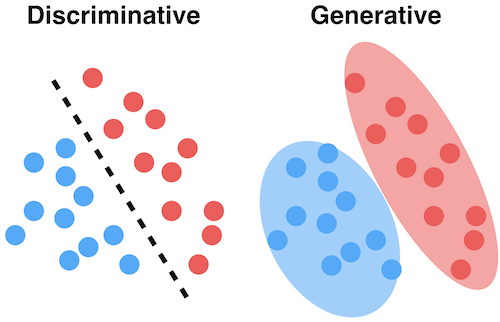
\includegraphics[width=0.65\columnwidth]{figures/generative_discriminative.png}
	\caption{abra alatti szoveg}
\end{figure}

A diszkriminatív modellek a statisztikai osztályozásban használt modellek egy osztályára vonatkozik, amelyet főként felügyelt gépi tanulási feladatokra használnak. Az ilyen típusú modelleket feltételes modelleknek is nevezik, mivel megtanulják az osztályok vagy címkék elhatárolását egy adathalmazban. A diszkriminatív modellek (akárcsak a szó szerinti értelemben) a feltételes valószínűség modellezése helyett elkülönítik az osztályokat, és nem tesznek feltételezéseket az adatpontokról. Ezek a modellek azonban nem képesek új adatpontok előállítására. Ezért a diszkriminatív modellek végső célja az egyes osztályok elkülönítése egymástól.

%----------
A generatív modellek a felügyelet nélküli tanulásban használatosak. Ezek a modellek képesek megtanulni a tanító minták valószínűségi eloszlását, majd tanítás után új minták generálására képesek. Ez a tulajdonság a gyakorlatban rendkívűl előnyös. 

A mély tanulásban használt modellek betanításához nagy mennyiségű, és megflelelő minőségű adatra van szükség, ezért az ezzel foglalkozó vállalatok rengeteg erőforrást áldoznak a tanítóminták begyűjtésére. Jellemzően manuális annotációra van szükség ami munkaigényes folyamat. Ez a megközelítés költséges, és nehezen skálázható. A jó minőségű adathoz tipikusan csak a nagyobb vállalatok képesek hozzájutni. A miatt generatív modellek használatával több válalat képes minőségi adatokat előállítani kevesebb mintából.

% ezt lehetne szövegesen kifejteni mert érdekes.
A generatív modelleknek számos felhasználási területe van, ezek közül néhány példa:
\begin{itemize} 
	\item Fotorealisztikus emberi arcképek generálására képes. [REF]
	\item Egy képet leíró szöveg alapján képes képet készíteni
	\item MRI kép rekonstruációra alkalmas
	\item Az adathalmazban ritkán előforduló adatok generálását tudja, ami kiegyensúlyozhatja az adatot.
	\item Realisztikusan képes utánozni az emberi hangot
\end{itemize}


% ~~~
% The learning models in machine learning can be classified into two sub-categories, Discriminative models and Generative models. Discriminative models classify input data; i.e., given the features of an instance of data, they predict a label or category to which that data belongs. In Supervised Learning, the classification algorithms/models are examples of discriminative models.

% Generative Modelling is an unsupervised learning task in machine learning that involves generating new data samples from the probability distribution of training data. Given some data, the aim is to have a model for the underlying probability distribution of that data so that we can draw samples that are similar to our training data.

%~~~~~~~~~~
% Machine learning models can be classified into two types of models – Discriminative and Generative models. In simple words, a discriminative model makes predictions on the unseen data based on conditional probability and can be used either for classification or regression problem statements. On the contrary, a generative model focuses on the distribution of a dataset to return a probability for a given example.
%~~~~~~~~~~ (https://www.analyticsvidhya.com/blog/2021/07/deep-understanding-of-discriminative-and-generative-models-in-machine-learning/)

%~~~~~~~~~
Tegyük fel, hogy van egy adathalmazunk, amely emberi arcokról készült fényképeket tartalamz. Egy olyan modellt szeretnénk létrehozni, amely képes egy nem létező emberről arcképet generálni, ami mégis valóságosnak tűnik, mert a modell megtanulta az emberi arcot leíró általános szabályokat. Az ilyen feladatok megoldhatóak generatív modellezéssel. a \ref{fig:generative_model}. ábra egy tipikus generatív modellezési folyamatot mutat be.

\begin{figure}[h]
	\centering
	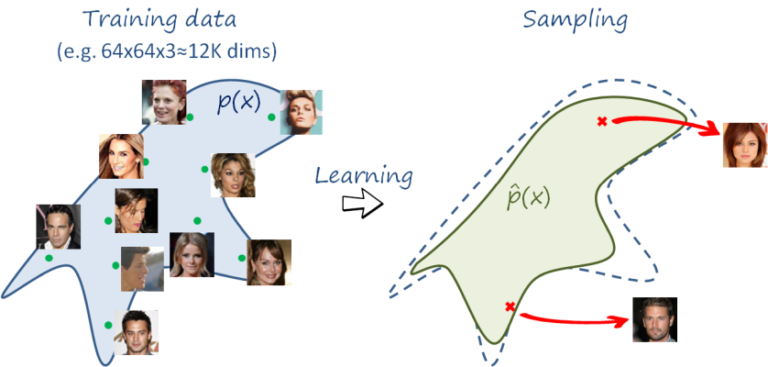
\includegraphics[width=0.9\columnwidth]{figures/generative_model_struct.png}
	\caption{abra alatti szoveg}
	\label{fig:generative_model}
\end{figure}

Először is szükségünk van egy adathalmazra, amely számos mintát tartalmaz az általunk generálni kivánt dologról. Az adathalmaz egyes elemeit megfigyeléseknek (observation) is nevezik. Minden megfigyelés sok jellemzőből (feature) áll amelyek képek esetén az egyes pixelek értékeit jelentik. Célunk egy olyan modell létrehozása, amely képes olyan új megfigyeléseket generálni, amelyek jellemzői jól közelítik az az eredeti adathalmazban lévő jellemzőket. Képgenerálás esetén ez egy rendkívűl nehéz feladat, mivel az egyes pixel értékek rengeteg lehetséges értéket vehetnek fel, és ezek közül csak relatíve kevés konfiguráció felel meg annak a képnek amit mi generálni szeretnénk.

A generatív modellek sztochasztikus jellegűnek kell lennnie, nem pedig determinisztikusnak. Ha a modellünk csupán egy fixált számítást végezne, példáuk az adathalmaz minden egyes pixelének átlagát számolná, akkor a modell minden alkalommal ugyanazt a kimenetet eredményezi. Így a generatív modellek szükségszerűen tartalmaznia kell egy sztochasztikus (véletlenszerű) elemet, amely befolyásolja a modell által generált mintákat.

Más szavakkal, létezik egy ismeretlen valószínűségi eloszlás, amely megmagyarázza, hogy az egyes képek miért találhatóak a mintakészletünkban, még más képek nem. A gyakorlatban nem ismerjük a tényleges valószínűségi eloszlást, ezért azt csak közelíteni tudjuk a megfigyelések mintájából. A generatív modellek célja az, hogy ezt az eloszlást minél jobban közelítse. A modell tanítása után az eloszlást mintavételezve olyan megfigyeléseket kaphatunk, amelyek az eredeti adathalmaz elemeihez nagyon hasonlóak.

%------------
% In practice, we may not be able to assess or observe all possible outcomes of a random variable due to which we generally do not know the actual density function. In such conditions, we must rely on approximating the density function from a sample of observations. Approximating a density function using a sample of observations is referred to as ‘Density estimation’.  Learning density estimate from the training samples is fundamental to generative models.
%~~~~~~~~~~~
% Suppose we have a dataset containing images of horses. We may wish to build a model that can generate a new image of a horse that has never existed but still looks real because the model has learned the general rules that govern the appearance of a horse. This is the kind of problem that can be solved using generative modeling. A summary of a typical generative modeling process is shown in Figure 1-1.

% First, we require a dataset consisting of many examples of the entity we are trying to generate. This is known as the training data, and one such data point is called an observation. Each observation consists of many features—for an image generation problem, the features are usually the individual pixel values. It is our goal to build a model that can generate new sets of features that look as if they have been created using the same rules as the original data. Conceptually, for image generation this is an incredibly difficult task, considering the vast number of ways that individual pixel values can be assigned and the relatively tiny number of such arrangements that constitute an image of the entity we are trying to simulate.

% A generative model must also be probabilistic rather than deterministic. If our model is merely a fixed calculation, such as taking the average value of each pixel in the dataset, it is not generative because the model produces the same output every time. The model must include a stochastic (random) element that influences the individual samples generated by the model.

% In other words, we can imagine that there is some unknown probabilistic distribution that explains why some images are likely to be found in the training dataset and other images are not. It is our job to build a model that mimics this distribution as closely as possible and then sample from it to generate new, distinct observations that look as if they could have been included in the original training set.
%~~~~~~~~~ (https://www.oreilly.com/library/view/generative-deep-learning/9781492041931/ch01.html)

%~~~~~~~~~
% Mathematically, generative models learn the joint probability distribution P(X,Y), whereas the discriminative models learn the posterior probability, P(Y|X), that is the probability of the label Y given the data X.
%~~~~~~~~~ (https://openai.com/blog/generative-models/)

%~~~~~~~~~~~~~~~~
% Because deep learning relies on the amount and quality of the data that is used to train it, companies spend a lot to get good image data. Typically, they use either expensive human annotation or other labor-intensive tasks, such as taking more photos of products or people. This approach is costly, and it doesn’t scale. Training computers to generate high-quality images can significantly reduce cost and stimulate business growth. One of the main challenges for AI is the lack of annotated or tagged data. High-quality annotated data is very costly, so only big or rich companies can get it. Using deep learning methods, such as those described in the paper, allows more companies to generate quality data from fewer samples.
%~~~~~~~~~~~~~~~~ (https://aws.amazon.com/blogs/machine-learning/combining-deep-learning-networks-gan-and-siamese-to-generate-high-quality-life-like-images/)

%~~~~~~~~~~~~~ some more from: (https://www.analyticsvidhya.com/blog/2021/07/deep-understanding-of-discriminative-and-generative-models-in-machine-learning/)

%----------------------------------------------------------------------------
% \subsubsection{Generative model types}


Matematikailag, az adathalmaz elemei $x_1, \dots, x_n$ a valódi háttéreloszlásból $p(x)$ lettek mintavételezve. A \ref{fig:data_distribution}. ábrán a kék háttérrel jelölt terület azon részét mutatja, amely nagy valószínűséggel (bizonyos küszöbérték felett) valódi képeket tartalmaz, és fekete pontok jelzik adatpontjainkat (mindegyik egy kép az adatkészletünkben). Modellünk egy becsült elosztást is leír $\hat{p}_{\theta}(x)$ (zölddel jelölt az ábrán) amelyet implicit módon úgy határozunk meg, hogy pontokat veszült egy egység Gauss eloszlásból (pirossal jelölt), és feltérképezzük őket egy determinisztijus neurális hálón - ami a generatív modellünk (sárga). A Neurális hálózat $\theta$ paraméterekkel rendelkezik, amelyeket módosítva megváltozik a generált képek eloszlását. Célunk olyan $\theta$ paraméterek meghatározása, amelyek egy olyan eloszlást hoznak létre, amely jól közelíti a valódi adateloszlásunkat. A $\theta$ paraméterek meghatározása egy iteraív folyamat, véletlenszerű értékekkel inicializálva, majd a tanítás során a paraméterek megváltoztatásával egyre jobban közelíti a becsült eloszlás a valódi adateloszlást.

\begin{figure}[ht]
	\centering
	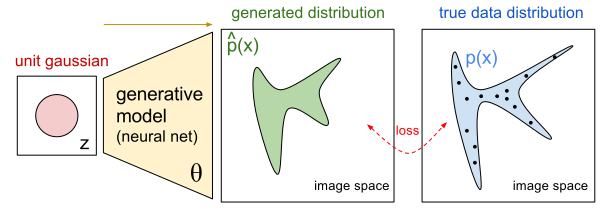
\includegraphics[width=1\columnwidth]{figures/generative_model_math.png}
	\caption{abra alatti szoveg}
	\label{fig:data_distribution}
\end{figure}

%-------
% Now, it is not always possible for our machine to learn the true distribution of the data, for this, we take the help of a powerful neural network which can help make the machine learn the approximate true distribution of the data. The neural networks we use as generative models have parameters which are smaller than the amount of data we have as training dataset. The models are forced to discover the distribution in order to generate data.
%-------

A generatív modellek általában kétféle sűrűségbecslést használnak. Explicit Sűrűségbecslés (EDE), és Implicit Sűrűségbecslés (IDE). Az EDE-ben előre meghatározott sűrűségfüggvényeket használnak a megfigyelések és valószínűségeik közötti kapcsolat közelítésére. Ezek a függvények paramétereik változtatásával illeszthetőek a megfigyelésekre. Például normál eloszlás két paramétere: várható érték és szórás állításával illeszthető az adatra. Aze IDE-ben nem előre meghatározott sűrűségfüggvényeket használnak, hanem egy algoritmust használnak a valószínűségi eloszlás közelítésére. Ennek egy példája kernel sűrűségbecslés. Bár az IDE módszerek is paramétereket használnak a közelítéshez, ezeket nem lehet közvetlenül manipulálni mint az EDE esetén. A \ref{fig:gen_models_tax}. ábra a különböző generatív modellek rendszerezését mutatja be az alkalmazott sűrűségbecslés típusa szerint.

% Generative Adversial Network (GAN) is an Implicit density based generative model. Variational Autoencoder (VAE) and Boltzmann Machine (BM) are the explicit density based generative models.  

% Two types of density estimations are generally used in generative models; Explicit Density Estimation (EDE) and Implicit Density Estimation (IDE). In EDE, predefined density functions are used to approximate the relationship between observations and their probability. The observed data is fit to predefined function by manipulating a fixed set of parameters of the function. An example is trying to fit given data to normal distribution using mean and the standard deviations of the samples. This type of density estimation is also known as parametric density estimation. In IDE, predefined density functions are not used. Instead an algorithm is used to approximate the probability distribution of the data. Kernel density approximation is an example of this type. Though the IDE methods use parameters for approximation, they cannot be directly manipulated the way they are in EDE. Figure 3 shows the taxonomy of different generative models based on the type of density estimation used.

\begin{figure}[ht]
	\centering
	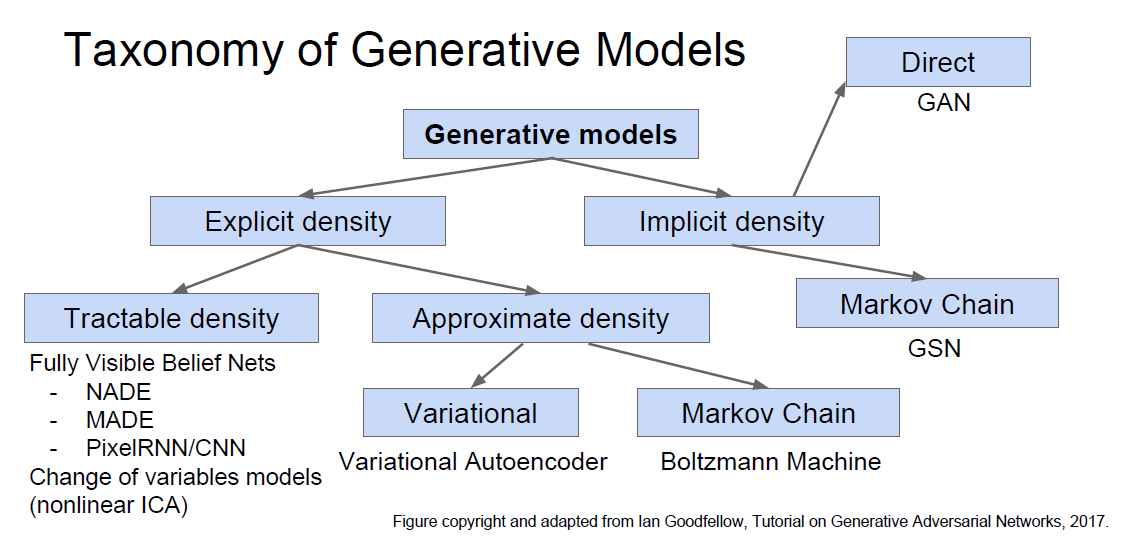
\includegraphics[width=0.8\columnwidth]{figures/generative_model_taxonomy.png}
	\caption{abra alatti szoveg}
	\label{fig:gen_models_tax}
\end{figure}


%----------------------------------------------------------------------------
%----------------------------------------------------------------------------
\subsection{Boltzman gépek}

A következő részben a generatív modellek egyik fajtáját: a Boltzman gépet (BM) működését, illetve annak egyik változatát, a Restricted Boltzman gépet (RBM) mutatom be, de előtte néhány alapvető fogalmat mutatok be amik szükségesek a BM megértéséhez.

% A jelenlegi cikkben a generatív modellekre fogunk összpontosítani, különösen a Boltzmann Machine (BM), népszerű változata a Restricted Boltzmann Machine (RBM), az RBM működésére és néhány alkalmazására. Mielőtt elmélyülne a BM részleteiben, megvitatunk néhány alapvető fogalmat, amelyek elengedhetetlenek a BM megértéséhez.

% In the current article we will focus on generative models, specifically Boltzmann Machine (BM), its popular variant Restricted Boltzmann Machine (RBM), working of RBM and some of its applications. Before deep-diving into details of BM, we will discuss some of the fundamental concepts that are vital to understanding BM. 

% BMs are useful to extract latent space from the data. The difference is in the architecture, the representation of the latent space and the training process. 

%----------------------------------------------------------------------------
\subsubsection{Markov-lánc}

A matematikában a Markov-lánc egy olyan diszkrét sztochasztikus folyamatot jelent, amely Markov-tulajdonságú. Nevét egy orosz matematikusról, Andrej Markovról kapta, aki hírnevét a tudomány ezen ágában végzett kutatásaival szerezte. Markov-tulajdonságúnak lenni röviden annyit jelent, hogy adott jelenbeli állapot mellett, a rendszer jövőbeni állapota nem függ a múltbeliektől. Másképpen megfogalmazva ez azt is jelenti, hogy a jelen leírása teljesen magába foglalja az összes olyan információt, ami befolyásolhatja a folyamat jövőbeli helyzetét. A \ref{fig:markov}. ábra mutat egy példát a Markov-láncra. A véletlenszerűen sétáló személy helyzete a $t+1$ pillanatban a $t$ aktuális állapottól függ, és nem a korábbi állapotoktól $(t-1, t-2,\dots)$. Ezt a viselkedést Markov tulajdonságnak nevezik.

% A Markov chain is a probabilistic model used to estimate a sequence of possible events in which the probability of each event depends only on the state attained in the previous event.  In a Markov chain, the future state depends only on the present state and not on the past states. An example of Markov’s process is show in figure 4.  The position of the randomly walking person at instant t+1 is dependent on the current state t and not on the previous states (t-1, t-2, …..). This behavior is referred to as Markov property.

\begin{figure}[ht]
	\centering
	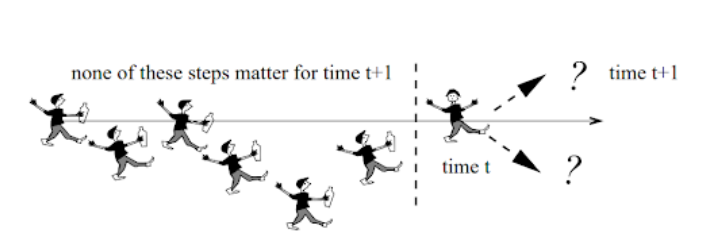
\includegraphics[width=1\columnwidth]{figures/markov_chain.png}
	\caption{abra alatti szoveg}
	\label{fig:markov}
\end{figure}


%----------------------------------------------------------------------------
\subsubsection{Grafikus modell}

A grafikus valószínűségi modell egy grafikus ábrázolás, amivel véletlen változók közötti feltételes valószínűséget lehet kifejezni. A grafikus modellnek két fő komponense van: csúcsok és élek. A csúcsok a véletlen változó állapotát jelzik, míg az élek az átalakulás irányát. Az ilyen gráfoknak két fő típusa van: irányított és irányítatlan. A \ref{fig:graph}. ábrán látható példán egy csecsemő táplálkozási szokásainak Markov folyamatának irányítatlan grafikus modelljét láthatjuk. A baba következő étkezésének kiválasztása kizárólag attól függ, hogy mit eszik most, és nem attól, amit korábban evett.

\begin{figure}[ht]
	\centering
	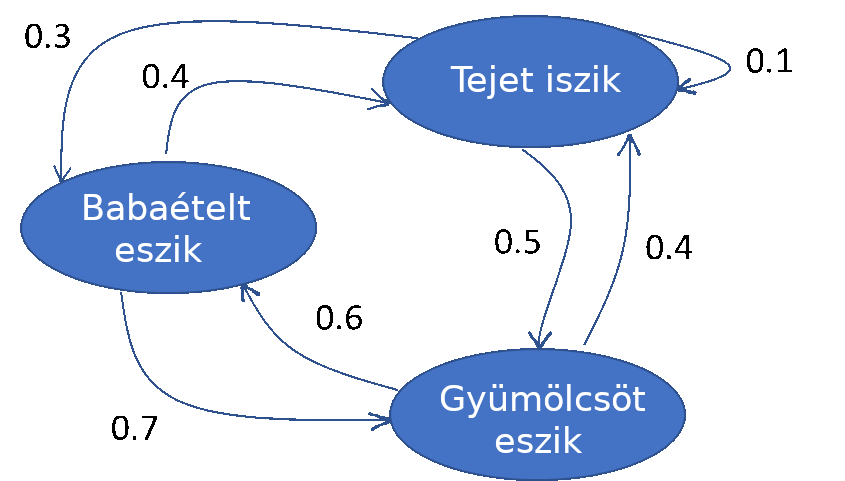
\includegraphics[width=0.7\columnwidth]{figures/graph_example.png}
	\caption{abra alatti szoveg}
	\label{fig:graph}
\end{figure}

%https://en.wikipedia.org/wiki/Graphical_model

% A grafikonmodell segítségével jelezhetjük a baba választását a következő étkezéshez a valószínűségekkel együtt. A baba következő étkezésének kiválasztása kizárólag attól függ, hogy mit eszik most, és nem attól, amit korábban evett. Annak valószínűségét, hogy egy adott ételt választanak a következő étkezéshez, történelmi megfigyelések alapján számítják ki.

% A graphical probabilistic model is a graphical representation used to expresses the conditional dependency between random variables. A graphical model has two components in it; Vertices and edges. The vertices indicate the state of random variable and the edge indicates direction of transformation. The two main types of computational graphs; directed and undirected. Figure 6 shows an undirected graphical model of a Markov process of diet habit of a baby. The graph model is used to indicate a baby’s choice for the next meal with the associated probabilities. The baby’s choice of next meal depends solely on what it is eating now and not what it ate earlier. The probability of choosing a specific food for next meal is calculated based on historic observations.

%-------

Egy Markov tulajdonsággal rendelkező irányítatlan gráf által leírt valószínűségi változók halmazát Markov hálózatnak (Markov Random Field az angol szakirodalomban). A Boltzman gépek is a MRF-ek közé tartozik.

A Boltzman gép egy probabilisztikus generatív irányítatlan gráfmodell, amely kielégíti a Markov tulajdonságot. A BM-ek megtanulják a tanító minták eloszlását, majd abból új mintákat tudnak generálni. A BM rendelkezik bemeneti réteggel (látható réteggel) és egy vagy több rejtett réteggel. Kimeneti rétege nincs. A \ref{fig:bm}. ábrán láthatunk egy tipikus egy rejtett réteget tartalmazó Boltzman gépet.

% A Markov tulajdonsággal rendelkező és egy nem irányított gráf által leírt véletlen változók halmazát Markov Random Field (MRF) vagy Markov hálózatnak nevezzük. Más szavakkal, egy véletlen mező Markov véletlenszerű mező, ha kielégíti Markov tulajdonságát. A BM egyfajta MRF.

% A Boltzmann -gép (BM) egy valószínűségi generatív irányítatlan gráfmodell, amely kielégíti Markov tulajdonságát. A BM -ek megtanulják a valószínűségi sűrűséget a bemeneti adatoktól az új minták generálásáig azonos eloszlásból. A BM rendelkezik bemeneti vagy látható réteggel és egy vagy több rejtett réteggel. Nincs kimeneti réteg. A 6. ábra egy rejtett rétegű BM tipikus architektúráját mutatja.

% A set of random variables having Markov property and described by an undirected graph is referred to as Markov Random Field (MRF) or Markov network. In other words, a random field is said to be a Markov random field if it satisfies Markov property. BM is a type of MRF.

% We now have a grasp on some of the fundamental concepts to understand BM. A Boltzmann Machine (BM) is a probabilistic generative undirected graph model that satisfies Markov property. BMs learn the probability density from the input data to generating new samples from the same distribution. A BM has an input or visible layer and one or several hidden layers. There is no output layer. Figure 6 shows a typical architecture of a BM with single hidden layer. 

A hálózat neuronjai megtanulnak sztochasztikus döntéseket hozni akkór, hogy be vagy kikapcsoljanak a tanítás során látott mintáknak megfelelően. Így a BM-ek fel tudják fedni a tanító adatok összetett mögöttes mintázatait. Lényeges különbség a BM és az egyéb neurális hálózat architektúrák között az, hogy a BM neuronjai nemcsak más rétegek neuronjaihoz kapcsolódnak, hanem ugyanazon a rétegen belüli neuronokhoz is, minden neuron kapcsolódik a hálózat összes többi neuronhoz. Ezt azt architektúrát Korlátlan Boltzman Gépnek nevezik, aminek a tanítása rendkívűl nehézkes és e miatt kevés gyakorlati haszna van. Az azonos rétegbeli idegsejtek közötti kapcsolatok megszüntetésével egy más architektúrát kapunk amit Korlátozott Boltzman Gépnek (RMB) hív a szakirodalom. A gyakorlatban az RBM-et használják, mert a hálót könyebb tanítani. A BM és RBM közötti különbséget a \ref{fig:bm}. ábra szemlélteti.

\begin{figure}[ht]
	\centering
	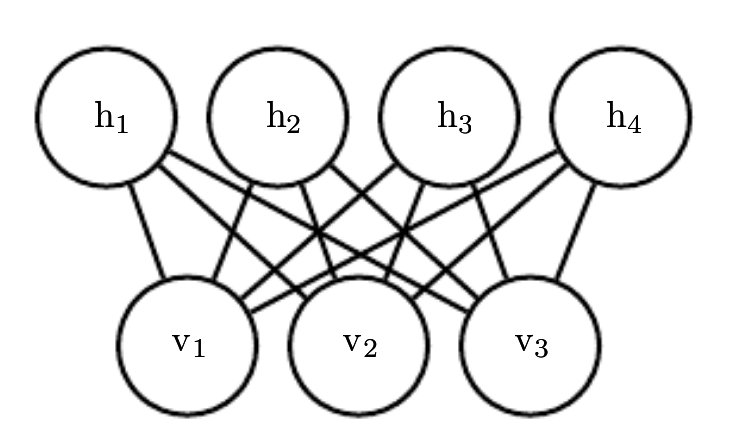
\includegraphics[width=0.50\columnwidth]{figures/RBM.png}
	\caption{A korlátozott Boltzman gép (RBM) egy kétirányú gráfon alapuló irányítatlan grafikus modell, aminek egyik részén a látható elemek vannak (v), a másik részén a rejtett elemek (h).}
	\label{fig:bm}
\end{figure}

% The neurons in the network learn to make stochastic decisions about whether to turn on or off based on the data fed to the network during training.  This helps the BM discover and model the complex underlying patterns in the data. A vital difference between BM and other popular neural net architectures is that the neurons in BM are connected not only to neurons in other layers but also to neurons within the same layer. Essentially, every neuron is connected to every other neuron in the network.  This imposes a stiff challenge in training a BM and this version of BM, referred to as ‘Unrestricted Boltzmann Machine’ has very little practical use. Eliminating the connections between the neurons in the same layer relaxes the challenges in training the network and such networks are called as Restricted Boltzmann Machine (RBM). In practice, RBMs are used in verity of applications due to simpler training process compared to BMs

% \subsubsection{Energy based model}
%~~~~~~~~
% Boltzmann Machines are primarily divided into two categories: Energy-based Models (EBMs) and Restricted Boltzmann Machines (RBM). When these RBMs are stacked on top of each other, they are known as Deep Belief Networks (DBN).
%~~~~~~~~~ (https://medium.com/machine-learning-researcher/boltzmann-machine-c2ce76d94da5)

%~~~~~~
% Energy is a term that may not be associated with deep learning in the first place. Rather is energy a quantitative property of physics. E.g. gravitational energy describes the potential energy a body with mass has in relation to another massive objected due to gravity. Yet some deep learning architectures use the idea of energy as a metric for the measurement of the model’s quality.
% One purpose of deep learning models is to encode dependencies between variables. The capturing of dependencies happens through associating of scalar energy to each configuration of the variables, which serves as a measure of compatibility. High energy means bad compatibility. An energy-based model tries always to minimize a predefined energy function. The energy function for the RBMs is defined as:

%equation :)
 
% As can be noticed the value of the energy function depends on the configurations of visible/input states, hidden states, weights, and biases. The training of RBM consists of the finding of parameters for given input values so that the energy reaches a minimum.
%~~~~~~ (https://medium.com/machine-learning-researcher/boltzmann-machine-c2ce76d94da5)

% \subsubsection{Training}
% ha kell még content
%----------------------------------------------------------------------------
\subsubsection{RBM alkalmazásai}

Az mély tanulás első napjaiban az RBM-eknek különféle feladatoknál alkalmazták, mint például dimenziócsökkentéshez, vagy ajánlórendszerekhez vagy természetes nyelv feldolgozásra. Néhány alkalmazási példa RBM-re:
\begin{itemize}
	\item Mintázat felismerés: Az RBM jellemzők kinyerésére (feature extraction) alkalmas mintázatfelismerési problémák esetén, amikor kézzel írott szöveg felismerése a cél. [REF]
	\item Anánlórendszerek: Az RBM-eket széles közben használják olyan feladatokra, ahol megjósolják, hogy mit érdemes ajánlani a felhasználónak ami számára hasznos lenne, és ezért szívesen használja az alkalmazást. Példa: filmajánlás, zeneajánló. [REF]
\end{itemize}

Azonban az utóbbi időkben a gyakorlatban az RBM-eket szinte teljesen felváltották a Generatív Adversarial Network-ök (GAN), vagy a Variational Autoencoderek (VAE).

% Pattern recognition : RBM is used for feature extraction in pattern recognition problems where the challenge is to understand the hand written text or a random pattern. 
% Recommendation Engines : RBM is widely used for collaborating filtering techniques where it is used to predict what should be recommended to the end user so that the user enjoys using a particular application or platform. For example : Movie Recommendation, Book Recommendation
% Radar Target Recognition : Here, RBM is used to detect intra pulse in Radar systems which have very low SNR and high noise.

% During the early days of deep learning, RBMs were used to build a variety of applications such as Dimensionality reduction, Recommender systems, Topic modelling. However, in recent times, RBMs have been almost replaced by Generative Adversarial Networks (GANs) or Variation Autoencoder (VAEs) in different machine learning applications.

%----------------------------------------------------------------------------
\subsection{Generatív Adversarial Network}
%----------------------------------------------------------------------------

A Generatív Adversarial Network (más néven GAN) az utóbbi évek egyik innovációja a mély tanulás területén. A GAN-okat eredetiel Ian Goodfellow és Yoshua Gengio vezették be a Montreali Egyetemen, 2014-ben. A GAN-ok célja egy eloszlás megtanulása, és abból új példányok generálása.

A GAN egy generatív modell, amelyben két neurális háló verseng egymással. Az első hálót generátornak nevezik. A generátor felelős új szintetikus minták előállításáért, amelyek hasonlítanak a tanító halmaz mintáihoz. A másik neurális hálót diszkriminátornak nevezik, aminek a feladata megkülönböztetni a valódi minták (tanító minta) illetve a generátor által létrehozott szintetikus minták között. A generátor célja becsapnia a diszkriminátort, míg a diszkriminátor megpróbál ennek ellenállni. A két háló versengéséből ered az ``adversarial'' elnevezés.

Az alábbi \ref{fig:gan_struct}. ábrán látható, hogy a generátor nem találkozik a tanító mintákkal, csupán véletlen zajt kap a bemenetére. A diszkriminátor hozzáfér a tanító adatokhoz osztályozás céljából. A generátor képes javítani a kimenetén kizárólag a diszkriminátortól kapott visszajelzés alapján (pozitív, ha a tanító mintával egyezik a kimenet, negatív ha nincs egyezés).

%~~~~~~~~~~~~~~~~~~
% Generative Adversarial Networks (a.k.a. GANs) represents one of the most exciting recent innovation in deep learning. GANs were originally introduced by Ian Goodfellow and Yoshua Bengio from the University of Montreal, in 2014.

% A GAN is a generative model in which two neural networks are competing in a typical game theory scenario. The first neural network is the generator, responsible of generating new synthetic data instances that resemble your training data, while its adversary, the discriminator tries to distinguish between real (training) and fake (artificially generated) samples generated by the generator. The mission of the generator is to try fooling the discriminator, and the discriminator tries to resist from being fooled. That’s why the system as a whole is described as adversarial.

% As shown in the figure below, the generator’s input is simply a random noise, while, only the discriminator has access to the training data for classification purposes. The generator keeps improving its output based, exclusively, on the feedback of the discriminator network (positive in case of match with training data and negative if there is no match). The goal for these generated data samples is to be the fair samples from the distribution of real data.
%~~~~~~~~~~~~~~~~~~
% Generative adversarial networks, also known as GANs are deep generative models and like most generative models they use a differential function represented by a neural network known as a Generator network. GANs also consist of another neural network called Discriminator network.

% A Generator network takes random noise as input and runs that noise through the differential function to transform the noise and reshape it to get a recognisable structure. The output of the generator seems like a real data point. The choice of the random input voice determines which data point will come out of the generator network. Running the generator network with many different input noise values produces many different realistic output data samples. The goal for these generated data samples is to be the fair samples from the distribution of real data.

\begin{figure}[ht]
	\centering
	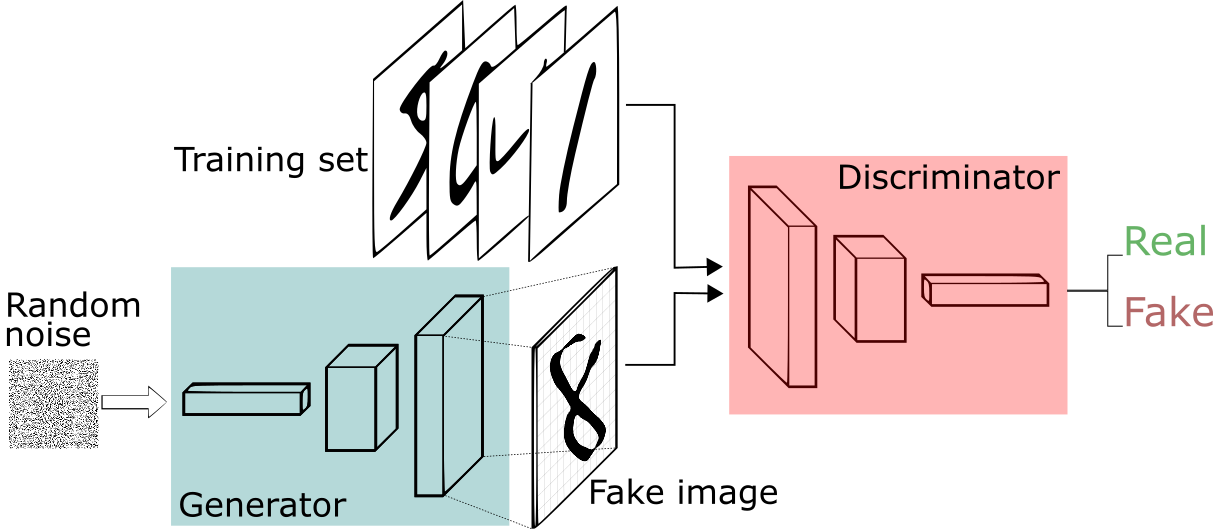
\includegraphics[width=0.9\columnwidth]{figures/gan_struct.png}
	\caption{abra alatti szoveg}
	\label{fig:gan_struct}
\end{figure}

\subsubsection{GAN tanítása}

A generátor be kell tanítani, mielőtt realisztikus mintákat képes létrehozni. Tegyük fel, hogy egy újonnan inicializált hálót használunk 200 kép előállítására, minden mintánál új random zaj bemenettel. Mivel a generatív modell tanítása felügyelet nélküli, nincsenek címkéink amivel össze lehetne vetni a háló kimenetét. Honnan tudjuk mégis, hogy milyen irányba kell módosítani a háló paramétereit, hogy javuljon a generált képek minősége? Egy generált kép ``jóságát'' nem külsőleg mondjuk meg (címke segítségével), hanem az dönti el, hogy sikerült-e átverni a diszkriminátort.

A diszkriminátor háló ad visszajelzést a generátornak tanulás során, hogy meg tudja tanulni az adott minták eloszlását. A diszkriminátor tipikusan egy osztályozó konvolúciós neurális háló ami képes megkülönböztetni a generált mintákat a valós mintáktól. A tanítás során a diszkriminátornak az esetek felében valódi mintákat, a másik felében szintetikus mintákat lát. A valós mintákhoz 1-hez közeli valószínűséget, hamis mintákhoz pedig 0-hoz közelit rendel. A generátor e közben megtanul olyan mintákat generálni, amelyekre a diszkriminátor 1-hez közeli kimenetet produkál, és valódi mintának minősítené azt. Idővel a generátor kénytelen egyre realisztikusabb kimeneteket előállítani, hogy meg tudja téveszteni a diszkriminátort. Ezzel a módszerrel egy felügyelet nélküli tanulási feladatot sikerül visszavezetni egy felügyelt tanulási feladatra.

% GAN -k közelítést használnak, ahol a második hálózat, a Diszkriminátor, a Generator -t vezeti, hogy a mintákat előállítsa az adott adatok valószínűségi eloszlásából. A diszkriminátor egy rendszeres neurális hálózat osztályozó, amely a valódi mintákat a generátor által generált hamis mintákból osztályozza. A képzési folyamat során a diszkriminátornak az idő felében valódi mintákat, a másik felében pedig hamis mintákat jelenítenek meg a generátorból. Valós mintákhoz 1 -hez közeli valószínűséget, hamis mintákhoz pedig 0 -hoz közeli valószínűséget rendel. Eközben a generátor olyan mintákat próbál kiadni, amelyeket a diszkriminátor közel egy valószínűséggel rendelne hozzá, és valódi mintáknak minősítené őket. Idővel a generátor kénytelen a reálisabb kimenetű mintákat előállítani a megkülönböztető félrevezetése érdekében. Ne feledje, hogy ez az ellentmondásos keret átalakította a nyers adatok és a minták nélküli felügyelet nélküli problémát az általunk létrehozott címkék által felügyelt problémává, azaz valódivá és hamisá.

% ~~~~~~~~~~~~
% The generator network needs to be trained before it can generate realistic data points as output. The training process for a generative model is different from that of the training process of a supervised model. For a supervised learning model, each input data is associated with its respective label whereas, for a generative model, the model is shown a lot of data samples and it makes new data samples that come from the same probability distribution.

% GANs use an approximation where a second network called the Discriminator guides the Generator to  generate the samples from the probability distribution of given data. The Discriminator is a regular neural network classifier that classifies the real samples from the fake samples generated by the Generator. During the training process, the Discriminator is shown real samples half of the time and fake samples from the Generator the other half of the time. It assigns a probability close to ‘1’ to real samples and the probability close to ‘0’ to fake samples. Meanwhile, the Generator is trying to output samples that the Discriminator would assign a probability of near one and classify them as real samples. Over time the generator is forced to produce the samples that are more realistic outputs in order to fool the Discriminator. Note that this adversarial framework has transformed an unsupervised problem with raw data and no samples into a supervised problem with labels we create, that is, real and fake. 

% ~~~~~~~~~~~~~ about training
% Suppose that we used a newly-initialized network to generate 200 images, each time starting with a different random code. The question is: how should we adjust the network’s parameters to encourage it to produce slightly more believable samples in the future? Notice that we’re not in a simple supervised setting and don’t have any explicit desired targets for our 200 generated images; we merely want them to look real. One clever approach around this problem is to follow the Generative Adversarial Network (GAN) approach. 
% Here we introduce a second discriminator network (usually a standard convolutional neural network) that tries to classify if an input image is real or generated. For instance, we could feed the 200 generated images and 200 real images into the discriminator and train it as a standard classifier to distinguish between the two sources. But in addition to that — and here’s the trick — we can also backpropagate through both the discriminator and the generator to find how we should change the generator’s parameters to make its 200 samples slightly more confusing for the discriminator. These two networks are therefore locked in a battle: the discriminator is trying to distinguish real images from fake images and the generator is trying to create images that make the discriminator think they are real. In the end, the generator network is outputting images that are indistinguishable from real images for the discriminator.
%~~~~~~~~~~~~~~ (https://openai.com/blog/generative-models/)

%~~~~~~~~~~~~~
% Generative adversarial networks (GANs), are a relatively new deep learning architecture for neural networks. They were pioneered by Ian Goodfellow and his colleagues at the University of Montreal in 2014. A GAN trains two different networks, one against the other, hence they are adversarial. One network generates an image (or any other sample, such as text or speech) by taking a real image and modifying it as much as it can. The other network tries to predict whether the image is “fake” or “real.” The first network, called the G network, learns to generate better images. The second network, the D network, learns to discriminate between the fake and real images. Its ability to discriminate improves over time. 
%~~~~~~~~~~~~~ (https://aws.amazon.com/blogs/machine-learning/combining-deep-learning-networks-gan-and-siamese-to-generate-high-quality-life-like-images/)


% ez az abra nem jön be az oldalról
\begin{figure}[ht]
	\centering
	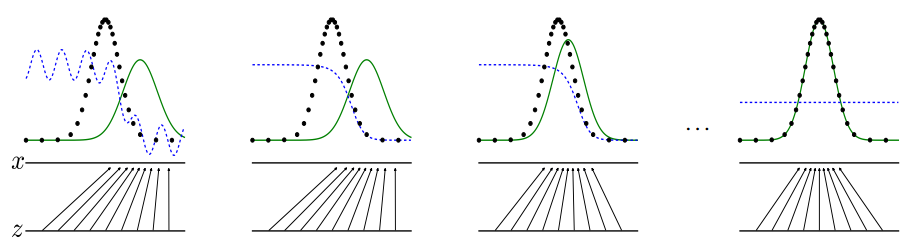
\includegraphics[width=1\columnwidth]{figures/gan_dist.png}
	\caption{Tanulás folyamata. Kék pontozott vonal jelöli a diszkriminátor eloszlását, zöld folytonos vonal a generált minták eloszlását, a fekete görbe pedig a tanító adat eloszlását. [REF]}
	\label{fig:gan_dist}
\end{figure}

A \ref{fig:gan_dist}. ábrán láthatjuk a GAN tanulásának folyamatát. A generátor $z$ véletlen zaj értéket kap bemenetre, és azt leképezi az $x$ kimeneti értékre. Az $x$ értékeinek eloszlása sűrűbbé válik, ahova több $z$ értéket képezünk le. A diszkriminátor magas értéket ad azokon a helyeken, ahol a valódi adatok sűrűsége nagyobb, mint a generált adatoké. A generátor a háló paramétereinek változtatásával módosítani tud a leképezésen, és így eléri, hogy az eloszlása a diszkriminátor gradiens irányába változzon. Végül a generátor eloszlása megegyezik a valós minták eloszlásával. Ekkor a diszkriminátor minden mintára 0,5-ös valószinűséget ad, mivel nem tudja megkülönböztetni a valós és generált mintákat.

% A generátor véletlen z zajértéket vesz fel, és leképezi x kimeneti értékre. A modell által ábrázolt x feletti valószínűségi eloszlás egyre sűrűbbé válik, ahol több z értéket leképezünk. A diszkriminátor magas értékeket ad ki mindenhol, ahol a valós adatok sűrűsége nagyobb, mint a generált adatoké. A generátor megváltoztatja az előállított mintákat, hogy felfelé haladjon a diszkriminátor által megtanult funkció mentén, és végül a generátor eloszlása megegyezik a valós adatok eloszlásával. Emiatt a diszkriminátor minden mintára 0,5 valószínűséget ad ki, mivel minden mintát ugyanolyan valószínűséggel hoz létre a valós adatkészlet, mint a generátort.

% The Generator takes random noise value z and maps them to output values x. The probability distribution over x represented by the model becomes denser wherever more values of z are mapped. The Discriminator outputs high values wherever the density of real data is greater than the density of generated data. The Generator changes the samples it produces to move uphill along the function learned by the Discriminator and eventually the Generator’s distribution matches the distribution of real data. Due to this, the Discriminator outputs the probability of 0.5 for every sample because every sample is equally likely to be generated by the real data-set as it is to be generated by the Generator.

% We can think of this process as a competition between police and counterfeiters. The Generator network is like a counterfeiter trying to produce fake money and pass it off as real. The police act as a Discriminator network and want to catch the counterfeiter spending the fake money but also do not want to stop people using real money. Over time the police get better at recognising fake money but at the same time, the counterfeiter also improves his techniques to produce fake currency. At some point, the counterfeiter makes exact replicas of the currency and the police can no longer discriminate between the real and fake money.

A GAN-oknak annak ellenére, hogy nemrég jelentek csak meg, gyakorlati hasznuk is van. Erre pár példa:
\begin{itemize}
	\item \textbf{StyleGan3}: Ez egy GAN-on alapuló neurális háló, amely képes az fotorealisztikus emberi arcképeket generálni. [REF] [https://nvlabs.github.io/stylegan3/]
	\item Egy 2018-as aukción egy GAN által ``festett'' kép több mint \$400 ezer dollárért kelt el [REF]
\end{itemize}

%----------------------------------------------------------------------------
\subsection{Generatív Autoenkóderek}

Az autoenkóderek olyan neurális hálók, ahol a kimeneti réteg mérete megegyezik a bemeneti réteg méretével. Az autoenkóder felügyelet nélküli tanulásra képes, feladata minél kisebb veszteséggel visszaállítsa a bemenetre érkező adatot, ezért replikátor neurális hálónak is nevezik. [REF]

% Autoencoder is a type of neural network where the output layer has the same dimensionality as the input layer. In simpler words, the number of output units in the output layer is equal to the number of input units in the input layer. An autoencoder replicates the data from the input to the output in an unsupervised manner and is therefore sometimes referred to as a replicator neural network.

% Az automatikus kódolók a bemenet minden dimenzióját úgy rekonstruálják, hogy átviszik a hálózaton. Lehet, hogy triviálisnak tűnik a neurális hálózat használata a bemenet replikálására, de a replikációs folyamat során a bemenet mérete kisebbre csökken. A neurális hálózat középső rétegei kevesebb egységgel rendelkeznek, mint a bemeneti vagy kimeneti rétegek. Ezért a középső rétegek tartják a bemenet csökkentett ábrázolását. Belsőleg rejtett réteggel rendelkezik, amely leírja a bemenet ábrázolásához használt kódot. A kimenet a bemenet ezen csökkentett ábrázolásából rekonstruálódik.

% The autoencoders reconstruct each dimension of the input by passing it through the network. It may seem trivial to use a neural network for the purpose of replicating the input, but during the replication process, the size of the input is reduced into its smaller representation. The middle layers of the neural network have a fewer number of units as compared to that of input or output layers. Therefore, the middle layers hold the reduced representation of the input. Internally, it has a hidden layer that describes a code used to represent the input. The output is reconstructed from this reduced representation of the input.

A háló tartalmaz egy $\textbf{h}$ rejtett réteget, ami a bemenet belső leképezését tárolja. A háló két részből tevődik össze: egy kódoló függvényből $\textbf{h} = f(\textbf{x})$, és egy dekódolóból, amely rekonstruálja a bemenetet $\textbf{r} = g(\textbf{h})$. Ha az autoenkóder egyszerűen megtanulná a $g(f(\textbf{x})) = \textbf{x}$ függvényt, az nem lenne túl hasznos, ezért a kódolót úgy tervezték, hogy képtelenek legyenek a bemenetet tökéletesen másolni. A kódolót úgy korlátozzák, hogy a középső rejtett réteg kevesebb neuront tartalmaz mint a bemeneti réteg. Ennek hatására a kódoló kénytelen priorizálni, hogy a bemenet mely jellemzőit érdemes másolni, így képes megtanulni az adatok hasznos tulajdonságait.

Az autoenkóderek tipikus felépítése: (látsd: \ref{fig:autoenc_struct}. ábra).

% A hálózat két részből tevődik össze: egy anenkódoló függvény = f (x) és egy dekódoló, amely rekonstrukciót eredményez = g (h). Ezt az architektúrát a 14.1. Ábra mutatja be. Ha egy automatikus kódolónak sikerül egyszerűen megtanulnia a setg (f (x)) = x mindenhol, akkor ez nem különösen hasznos. Ehelyett az automatikus kódolókat úgy tervezték, hogy képtelenek legyenek megtanulni tökéletesen másolni. Általában olyan módon korlátozzák őket, amelyek lehetővé teszik számukra, hogy csak hozzávetőlegesen másoljanak, és csak olyan adatokat másoljanak be, amelyek hasonlítanak az edzési adatokhoz. Mivel a modell kénytelen priorizálni, hogy a bemenet mely aspektusait kell másolni, gyakran megtanulja az adatok hasznos tulajdonságait

%~~~~~~~~~~~~~~~~~~~~~~~
% Internally, it has a hidden layerhthat describes acodeused torepresent the input. The network may be viewed as consisting of two parts: anencoder function=f(x) and a decoder that produces a reconstructionr=g(h).This architecture is presented in figure 14.1. If an autoencoder succeeds in simplylearning to setg(f(x)) =xeverywhere, then it is not especially useful. Instead,autoencoders are designed to be unable to learn to copy perfectly. Usually they are restricted in ways that allow them to copy only approximately, and to copy onlyinput that resembles the training data. Because the model is forced to prioritize which aspects of the input should be copied, it often learns useful properties of thedata
  
%~~~~~~~~~~~~~~~~~~~~~~ (https://www.deeplearningbook.org/contents/autoencoders.html)

% An autoencoder consists of three components:

\begin{figure}[ht]
	\centering
	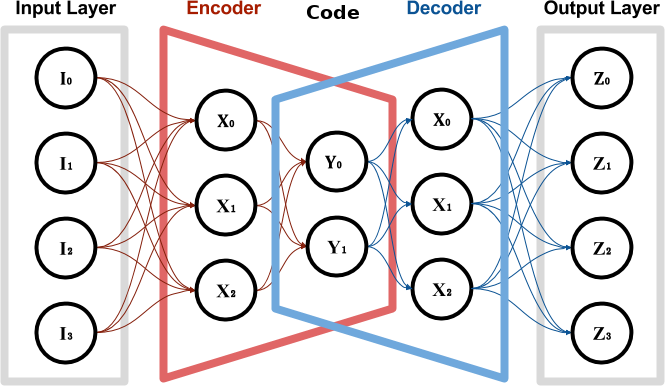
\includegraphics[width=0.8\columnwidth]{figures/autoenc.png}
	\caption{Az autoenkóder részei: enkóder, kód és dekódoló}
	\label{fig:autoenc_struct}
\end{figure}

\begin{itemize}
	\item \textbf{Kódoló}: A kódoló egy előrecsatolt, teljesen kapcsolt neurális háló, amely a bemenetet látens térbeli reprezentációba tömöríti. A bemeneti képet tömörített ábrázolásként kódolja csökkentett méretben.
	\item \textbf{Kód}: A hálózat ezen része tartalmazza a dekódolóba táplált bemenet csökkentett ábrázolását. (más néven látens változók).
	\item \textbf{Dekódoló}: A dekódoló a kódolóhoz hasonló struktúrájú előrecsatolt háló. Feladata kód alapján a bemenet visszaállítása.
\end{itemize}

Az autoenkóderek évtizedek óta ismertek a neurális hálózatok világában [REF]. Míg eleinte az autoenkódereket dimenziócsökkentéshez, vagy jellemző tanuláshoz használták, a közelmúltban a generatív modellezésben is előtérbe került. Az első komoly generatív tulajdonsággal rendelkező autoenkódert a variációs autoenkóder megjelenése hozta.

% A modern autókódolók a determinisztikus funkciókon túli kódoló és dekódoló ötletét a sztochasztikus leképezésekre (h | x) és pdekódolókra (x | h) általánosították. Az automatikus kódolók ötlete évtizedek óta része a neurális hálózatok történelmi tájának (LeCun , 1987; Bourlard és Kamp, 1988; Hinton és Zemel, 1994). Hagyományosan az automatikus kódolókat használták a dimenziócsökkentéshez vagy a funkciók tanulásához. A közelmúltban az autokódolók és a változó modellek közötti elméleti kapcsolatok az autokódolókat a generációs modellezés előtérébe hozták.

% Modern autoencoders have generalized the idea of an encoder and a de-coder beyond deterministic functions to stochastic mappingspencoder(h | x) andpdecoder(x | h).
% The idea of autoencoders has been part of the historical landscape of neuralnetworks for decades (LeCun, 1987; Bourlard and Kamp, 1988; Hinton and Zemel,1994). Traditionally, autoencoders were used for dimensionality reduction orfeature learning. Recently, theoretical connections between autoencoders andlatent variable models have brought autoencoders to the forefront of generativemodeling

\subsubsection{Variációs autoenkóderek}

A variációs autoenkóder (VAE) megjelenése nem túl régi, 2014-ben publikálták először [REF]. Bár mély neurális háló alapú autoenkóderek korábban is léteztek, mint generatív modell rosszul teljesítettek. Később azonban képgenerálás [REF], és megerősítéses tanulás [REF] területén is előremutató eredmények születtek.

% Az első komoly generatív tulajdonsággal rendelkező autóenkóder, a Variációs Au- tóenkóder (továbbiakban VAE) megjelenése nem túl régi: [25] [26] pulikálták elő- ször 2014-ben. Bár mély mesterséges háló alapú autóenkóderek előtte is léteztek, mint generatív modell azonban rosszul teljesítettek. Később azonban a képgenerálás, és a megerősítéses tanulás [27] területén is előremutató eredmények születtek.

%We add a constraint on the encoding network, that forces it to generate latent vectors that roughly follow a unit gaussian distribution. It is this constraint that separates a variational autoencoder from a standard one.

%TODO ezt újraírni h érthető legyen
A variációs autoenkóder annyiban tér el a standard autoenkódertől, hogy adunk egy megkötést a kódolónak, aminek hatására a generált látens változók vektora ($\textbf{h}$) közel követik a normál eloszlást. Ebben az esetben a normál eloszlás $N(\mu,\sigma)$ várható értéke ($\mu$) és szórása ($\sigma$) leírja a látens változók eloszlását. Ekkor az enkóder és dekóder nem determenisztikus hanem sztohasztikus jellegű. Ez a megkötés azért hasznos számunkra, mert normál eloszlásból könnyen tudunk mintavételezni, ami megkönnyíti az új képek generálását. 

% Új képek létrehozása most egyszerű: mindössze annyit kell tennünk, hogy mintát veszünk egy látens vektorból a gauss -egységből, és átadjuk a dekódolónak. A gyakorlatban kompromisszum van a hálózatunk pontossága és a látens változóinak közelítő egységei között.

%~~~~~~~~~~~~~~
% There's a simple solution here. We add a constraint on the encoding network, that forces it to generate latent vectors that roughly follow a unit gaussian distribution. It is this constraint that separates a variational autoencoder from a standard one.

% Generating new images is now easy: all we need to do is sample a latent vector from the unit gaussian and pass it into the decoder. In practice, there's a tradeoff between how accurate our network can be and how close its latent variables can match the unit gaussian distribution.
%~~~~~~~~~~~~~~ (https://kvfrans.com/variational-autoencoders-explained/)

A VAE működését könyebb egy példán keresztül bemutatni. Tegyük fel, hogy van egy képünk egy emberi arcról. A betanított háló ez a kép alapján képes látens változó vektort kinyerni a képből, ami az arcot leíró fontos jellemzőkből áll. Erre mutat egy példát a \ref{fig:vae_face}.ábra.

% Let us understand how we are generating new data. Let’s say we have the image of a celebrity face from which our encoder model has to recognize important features mentioned below. 

\begin{figure}[ht]
	\centering
	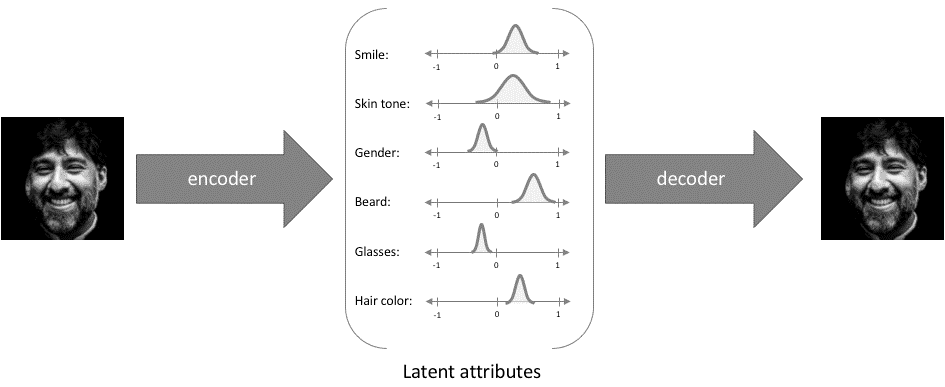
\includegraphics[width=1\columnwidth]{figures/autoenc_latent.png}
	\caption{Látens változók kinyerése a bemeneti arcképből.}
	\label{fig:vae_face}
\end{figure}

Mint a fenti ábrán látjuk, minden jellemzőhöz tartozik egy valószínűségi eloszlás. Miben különböznem az arcok? Megfogalmazhatunk pár ilyen jellemzőt, mint a bőrszín, haj színe, szemek távolsága, stb. Ezen jellemzőkből álló vektor leírhat egy emberi arcot. Eltérő arcoknál a jellemzők értékei mások lesznek, de jellemzők listája ugyanaz marad. Az autoenkóderek nem feltétlenül ilyen ember által könnyen értelmezhető jellemzőket nyer ki az arcokból, hanem azok ennél a példánál absztraktabbak.

Célunk, hogy új képeket állítsunk elő az arcképekből álló tanító mintahalmaz alapján. Feltéve, hogy a bemeneti adataink normál eloszlást követnek, új képek létrehozásához mindössze annyit kell tennünk, hogy normál eloszlásból mintavételezünk egy látens változó vektort. Ezt megadjuk a dekódolónak, ami a vektor alapján generálni tud egy új képet.

%TODO ezt kifejteni ha kell még content, ha nem akkor komment
A VEA számos területen alkalmazott, ezek közül egy példa az úgynevezett ``deepfake'' előállítása, ami lényegében abból áll, hogy egy személy arcát alakítják át úgy, hogy egy másik személy vonásait utánozza. [REF]

% This novel technique allows generating so-called deepfakes, which actually morph a person’s face to mimic someone else’s features, although preserving the original facial expression.

% With every feature, we have a probability distribution. Our goal is to produce new data from the current data or a new face from the current face. How do faces differ? Skin tone, eye colour, hair colour, and many other features are different. But overall, the list of the features remains the same. Since we have a facility with two probability distributions: mean and standard deviations, we have datasets of two new ranges to provide to the decoder.

% As our input data follows a normal distribution, we will be able to provide two variables: mean and variance in the latent space. We want to build a multivariate Gaussian model with the assumption of non-correlation in data which helps us result in a simple vector. Now, provide a set of random samples from mean and variance distributions from latent space to the decoder for the reproduction of data (image).

%if need more / better explonation: https://medium.com/analytics-vidhya/vae-generative-modelling-for-face-recognition-71e8ba16950c

%----------------------------------------------------------------------------
\subsection{Arcfelismerés neurális hálókkal}

asdfasf

\subsubsection{Mély metrika tanulás}

Similarity learning is an area of supervised machine learning in which the goal is to learn a similarity function that measures how similar or related two objects are and returns a similarity value. A higher similarity score is returned when the objects are similar and a lower similarity score is returned when the objects are different. Now let us see some use cases to know why and when similarity learning is used.

Consider a problem in which we have to train a model that can recognise all the students in a class to mark their attendance. We can use Image classification as discussed in the last section, we will collect data for all the students in the class and use them to train the model. After training the model, now we can recognise each student in the class. But what if we have a new student enrolled since we did not train the model on his data, it cannot recognise the new student. We will have to collect the new data and retrain the model, but training the model is expensive in terms of time and computation power. So we can pose this problem as similarity learning problem instead of a classification problem to solve this problem in an optimal way.

Now we will have a model that returns a similarity score instead of labels. So when a student enters, we can compare him with his photo and if the similarity score is higher than a certain threshold, we mark him present. Now if we have an unknown person who does not match any images in the data, the similarity score will be low and he won’t be marked present. Remember we don’t have to retrain the model in order to add new students, we just need his one image from which he can be compared.

Another example of similarity learning can be comparing the signature on the checks. These kinds of networks can also be used to compare the signature of the account holder to the signature on the check. If the similarity score is higher than the check is accepted and if the similarity score is low than the signature is most probably forged

We can also solve NLP problems using similarity learning. One popular problem it can solve is to recognise duplicate questions on popular forums such as Quora or StackOverflow on which thousands of questions are posted every hour. You might think that this is not that hard problem as all we have to do is compare words in these questions. You may be even right in some cases such as the questions “Where do you live?” and “Where are you living?” have almost same words in them so we can say that they are asking the same question. But if you consider another question “where are you going?”, this also looks similar to the last question but has an entirely different meaning. Even in some cases, the words may totally not match but the questions are the same such as “How old are you?” and “What is your age?” are exactly two same questions but have so common words. So here we train a network that returns a high similarity score when the questions are similar and a low similarity score when the questions are different.

Now how do we train a network to learn similarity? We use Siamese neural networks which is discussed next.

%----------------------------------------------------------------------------
\subsubsection{Sziámi hálók}

A Siamese neural network (sometimes called a twin neural network) is an artificial neural network that contains two or more identical subnetworks which means they have the same configuration with the same parameters and weights. Usually, we only train one of the subnetworks and use the same configuration for other sub-networks. These networks are used to find the similarity of the inputs by comparing their feature vectors.

\begin{figure}[ht]
	\centering
	
\includegraphics[width=0.65\columnwidth]{figures/abra.png}
	\caption{abra alatti szoveg}
\end{figure}

Consider the diagram above, the very first subnetwork takes an image as input and after passing through convolutional layers and fully connected layers,we get a vector representation of my face.Now the second face is actually the one I want to compare with the first face,so I pass this image through a network that is exactly the same with same weights and parameters.Now that we have two encodings F(A) and F(B), we will compare these two to know how similar the two faces are.

It is important to note that the F(A) and F(B) must be quite similar if both the inputs are similar which is the case in this example.And if the faces are different,we want F(A) and F(B) to be very different.So this is how we are going to train the network.

So how do we compare vectors F(A) and F(B) and when can we say that they are similar or different? We simply measure the distance between these vectors and if the distance between them is small than the vectors are similar and if the distance between is larger than the vectors are very different from one another.So we can define a distance function d, that can give us the distance between two vectors such as:

% d(A,B)=|| F(A) - F(B) ||<sup>2</sup>

So when A and B are the same person,d(A,B) is small and when A and B are different person d(A,B) is large.So we can form a loss functions around this.When A and B are a positive pair, i.e. are of a same person we can define the loss function exactly as L2 norm between F(A) and F(B).

% L(A,B)=|| F(A) - F(B) ||<sup>2</sup>

So when we minimise this loss function,we are actually minimizing the distance d(A, B). But for negative pairs(when two images in a pair are of different persons),we use a different kind of loss function known as hinge loss. When the two faces in a pair are different,we want F(A) and F(B) to have a distance greater than m, so if there is already a negative pair which has a distance greater than m between them,we don’t want to waste our effort by further making them apart.This is the reason we are using hinge loss instead of L2 loss.

% L(A,B)= max(0,m<sup>2</sup> - || F(A) - F(B) ||<sup>2</sup>)

So, this value is going to be zero when F(A) and F(B) are already distant apart(>m).

Now putting both of these losses together, we get a contrastive loss given as:

% L(A,B)= y|| F(A) - F(B) ||<sup>2 </sup> + (1-y)max(0,m<sup>2</sup> - || F(A) - F(B) ||<sup>2</sup>)<br>

So when A and B are the same person, we will have a label y equal to 1 and when A and B are different,y is equal to zero.

By using contrastive loss, we bring positive pairs together and negative pairs apart. But using this loss function we cannot learn ranking which means we are not able to say how much two pairs are similar to each other, we shall see how to do this in the next section.

%----------------------------------------------------------------------------
\subsubsection{Triplet veszteségfüggvény}

When using contrastive loss we were only able to differentiate between similar
and different images but when we use triplet loss we can also find out which
image is more similar when compared with other images. In other words, the
network learns ranking when trained using triplet loss.

When using triplet loss, we no longer need positive and negative pairs of
images. We need triplets of images in which we have an anchor image, a positive
image that is similar to anchor image and a negative image that is very
different from the anchor image as shown below:

Siamese network And now the architecture of the siamese network is as :

\begin{figure}[ht]
	\centering
	
\includegraphics[width=0.65\columnwidth]{figures/abra.png}
	\caption{abra alatti szoveg}
\end{figure}

Siamese network When computing the vectors for these images, we want the
vectors of anchor image and positive image to come closer and we want to make
increase the distance between anchor image and negative image.

The distance between anchor vector and the positive vector is given by:

% || F(A) - F(P) ||<sup>2</sup> Whereas the distance between anchor vector and the negative vector is given by:

% || F(A) - F(N) ||<sup>2</sup> As mentioned above, we want the anchor image and positive image to have less distance between them as compared to the distance between anchor image and negative image, therefore:

% || F(A) - F(P) ||<sup>2 </sup>< || F(A) - F(N) ||<sup>2</sup> So we can form the loss function as following:

% L(A,P,N)= max(0, || F(A) - F(P) ||<sup>2 </sup>< || F(A) - F(N) ||<sup>2</sup> +m) Where m is a margin as we also saw in the hinge function of the contrastive
loss. So if the positive image is already closer to the anchor than the negative
image than the function returns zero and there is no loss. But when the negative
image is closer to the anchor than the positive image, we are bringing a
positive image closer to the anchor. Remember that we are also using a margin
term m, so the anchor point and positive point are not coming very close to each
other, and only the distance between anchor image and positive image is smaller
as compared to the distance between anchor image and negative image up to a
margin m.

When training the network, we may face a problem with choosing the triplets. We
can choose triplets in which there is a lot of difference between the positive
image and negative image, thus the distance between the anchor image and
positive image is already quite smaller as compared to the distance between
anchor image and negative image. For example, when the positive image of a
person's face is completely different from the negative image like they can have
different hairstyles, face structure and many other factors. In this case, the
network is not able to learn completely and may not be able to differentiate on
the basis of more minute features such as eye shape, nose shape etc.\ This may
cause the model to not perform correctly when we compare two faces of different
persons that do not have much difference.

So to tackle this problem we use a concept called as hard negative mining in
which we train the network with hard cases. So we come up with such triplets in
which distance between positive image and anchor is somewhat equal to the
distance between negative image and anchor.
